\documentclass[12pt,]{article}
\usepackage[osf,sc]{mathpazo}
\usepackage{setspace}
\setstretch{1.1}
\usepackage{amssymb,amsmath}
\usepackage{ifxetex,ifluatex}
\usepackage{fixltx2e} % provides \textsubscript
\ifnum 0\ifxetex 1\fi\ifluatex 1\fi=0 % if pdftex
  \usepackage[T1]{fontenc}
  \usepackage[utf8]{inputenc}
\else % if luatex or xelatex
  \ifxetex
    \usepackage{mathspec}
  \else
    \usepackage{fontspec}
  \fi
  \defaultfontfeatures{Ligatures=TeX,Scale=MatchLowercase}
\fi
% use upquote if available, for straight quotes in verbatim environments
\IfFileExists{upquote.sty}{\usepackage{upquote}}{}
% use microtype if available
\IfFileExists{microtype.sty}{%
\usepackage{microtype}
\UseMicrotypeSet[protrusion]{basicmath} % disable protrusion for tt fonts
}{}
\usepackage[margin=1in]{geometry}
\usepackage{hyperref}
\hypersetup{unicode=true,
            pdftitle={Proposal: The Effect of U.S.~Military Aid on FDI},
            pdfauthor={Ben Horvath},
            pdfborder={0 0 0},
            breaklinks=true}
\urlstyle{same}  % don't use monospace font for urls
\usepackage{color}
\usepackage{fancyvrb}
\newcommand{\VerbBar}{|}
\newcommand{\VERB}{\Verb[commandchars=\\\{\}]}
\DefineVerbatimEnvironment{Highlighting}{Verbatim}{commandchars=\\\{\}}
% Add ',fontsize=\small' for more characters per line
\usepackage{framed}
\definecolor{shadecolor}{RGB}{248,248,248}
\newenvironment{Shaded}{\begin{snugshade}}{\end{snugshade}}
\newcommand{\AlertTok}[1]{\textcolor[rgb]{0.94,0.16,0.16}{#1}}
\newcommand{\AnnotationTok}[1]{\textcolor[rgb]{0.56,0.35,0.01}{\textbf{\textit{#1}}}}
\newcommand{\AttributeTok}[1]{\textcolor[rgb]{0.77,0.63,0.00}{#1}}
\newcommand{\BaseNTok}[1]{\textcolor[rgb]{0.00,0.00,0.81}{#1}}
\newcommand{\BuiltInTok}[1]{#1}
\newcommand{\CharTok}[1]{\textcolor[rgb]{0.31,0.60,0.02}{#1}}
\newcommand{\CommentTok}[1]{\textcolor[rgb]{0.56,0.35,0.01}{\textit{#1}}}
\newcommand{\CommentVarTok}[1]{\textcolor[rgb]{0.56,0.35,0.01}{\textbf{\textit{#1}}}}
\newcommand{\ConstantTok}[1]{\textcolor[rgb]{0.00,0.00,0.00}{#1}}
\newcommand{\ControlFlowTok}[1]{\textcolor[rgb]{0.13,0.29,0.53}{\textbf{#1}}}
\newcommand{\DataTypeTok}[1]{\textcolor[rgb]{0.13,0.29,0.53}{#1}}
\newcommand{\DecValTok}[1]{\textcolor[rgb]{0.00,0.00,0.81}{#1}}
\newcommand{\DocumentationTok}[1]{\textcolor[rgb]{0.56,0.35,0.01}{\textbf{\textit{#1}}}}
\newcommand{\ErrorTok}[1]{\textcolor[rgb]{0.64,0.00,0.00}{\textbf{#1}}}
\newcommand{\ExtensionTok}[1]{#1}
\newcommand{\FloatTok}[1]{\textcolor[rgb]{0.00,0.00,0.81}{#1}}
\newcommand{\FunctionTok}[1]{\textcolor[rgb]{0.00,0.00,0.00}{#1}}
\newcommand{\ImportTok}[1]{#1}
\newcommand{\InformationTok}[1]{\textcolor[rgb]{0.56,0.35,0.01}{\textbf{\textit{#1}}}}
\newcommand{\KeywordTok}[1]{\textcolor[rgb]{0.13,0.29,0.53}{\textbf{#1}}}
\newcommand{\NormalTok}[1]{#1}
\newcommand{\OperatorTok}[1]{\textcolor[rgb]{0.81,0.36,0.00}{\textbf{#1}}}
\newcommand{\OtherTok}[1]{\textcolor[rgb]{0.56,0.35,0.01}{#1}}
\newcommand{\PreprocessorTok}[1]{\textcolor[rgb]{0.56,0.35,0.01}{\textit{#1}}}
\newcommand{\RegionMarkerTok}[1]{#1}
\newcommand{\SpecialCharTok}[1]{\textcolor[rgb]{0.00,0.00,0.00}{#1}}
\newcommand{\SpecialStringTok}[1]{\textcolor[rgb]{0.31,0.60,0.02}{#1}}
\newcommand{\StringTok}[1]{\textcolor[rgb]{0.31,0.60,0.02}{#1}}
\newcommand{\VariableTok}[1]{\textcolor[rgb]{0.00,0.00,0.00}{#1}}
\newcommand{\VerbatimStringTok}[1]{\textcolor[rgb]{0.31,0.60,0.02}{#1}}
\newcommand{\WarningTok}[1]{\textcolor[rgb]{0.56,0.35,0.01}{\textbf{\textit{#1}}}}
\usepackage{graphicx,grffile}
\makeatletter
\def\maxwidth{\ifdim\Gin@nat@width>\linewidth\linewidth\else\Gin@nat@width\fi}
\def\maxheight{\ifdim\Gin@nat@height>\textheight\textheight\else\Gin@nat@height\fi}
\makeatother
% Scale images if necessary, so that they will not overflow the page
% margins by default, and it is still possible to overwrite the defaults
% using explicit options in \includegraphics[width, height, ...]{}
\setkeys{Gin}{width=\maxwidth,height=\maxheight,keepaspectratio}
\IfFileExists{parskip.sty}{%
\usepackage{parskip}
}{% else
\setlength{\parindent}{0pt}
\setlength{\parskip}{6pt plus 2pt minus 1pt}
}
\setlength{\emergencystretch}{3em}  % prevent overfull lines
\providecommand{\tightlist}{%
  \setlength{\itemsep}{0pt}\setlength{\parskip}{0pt}}
\setcounter{secnumdepth}{0}
% Redefines (sub)paragraphs to behave more like sections
\ifx\paragraph\undefined\else
\let\oldparagraph\paragraph
\renewcommand{\paragraph}[1]{\oldparagraph{#1}\mbox{}}
\fi
\ifx\subparagraph\undefined\else
\let\oldsubparagraph\subparagraph
\renewcommand{\subparagraph}[1]{\oldsubparagraph{#1}\mbox{}}
\fi

%%% Use protect on footnotes to avoid problems with footnotes in titles
\let\rmarkdownfootnote\footnote%
\def\footnote{\protect\rmarkdownfootnote}

%%% Change title format to be more compact
\usepackage{titling}

% Create subtitle command for use in maketitle
\newcommand{\subtitle}[1]{
  \posttitle{
    \begin{center}\large#1\end{center}
    }
}

\setlength{\droptitle}{-2em}

  \title{Proposal: The Effect of U.S.~Military Aid on FDI}
    \pretitle{\vspace{\droptitle}\centering\huge}
  \posttitle{\par}
    \author{Ben Horvath}
    \preauthor{\centering\large\emph}
  \postauthor{\par}
      \predate{\centering\large\emph}
  \postdate{\par}
    \date{November 1, 2018}

\usepackage{eulervm}

\begin{document}
\maketitle

Load libraries:

\begin{Shaded}
\begin{Highlighting}[]
\KeywordTok{library}\NormalTok{(dplyr)}
\KeywordTok{library}\NormalTok{(ggplot2)}
\KeywordTok{library}\NormalTok{(Hmisc)}
\KeywordTok{library}\NormalTok{(knitr)}
\KeywordTok{library}\NormalTok{(readxl)}
\KeywordTok{library}\NormalTok{(stringr)}
\KeywordTok{library}\NormalTok{(tidyr)}
\end{Highlighting}
\end{Shaded}

\hypertarget{introduction}{%
\section{Introduction}\label{introduction}}

I took a 200-level `methods in political science' class in the spring
semester of 2009, as part of an undergraduate degree in political
science. One assignment was to write a proposal for empirical research,
though we weren't required to necessarily carry out the analysis.

Biglaiser and DeRouen (2007) and Little and Leblang (2004) had found
that `the presence of U.S. troops serves as a ``catalyst'' for U.S.
outgoing foreign direct investment (FDI), that is, FDI follows the
flag.' My proposal, `The Effect of U.S. Military Aid on Foreign Direct
Investment Decisions,' was to test if U.S. arms exports had a similar
effect on FDI as U.S. troops. I located the appropriate data, and noted
a number of other variables that would need to be controlled for:
alliances, the presence of conflict, the Cold War and outliers like
Vietnam, regime type (democratic, autocratic, etc.), and population
size.

For methodology, I wrote, simply, `To test these associations, some kind
of regression would be used, with an appropriate significance test.' I
don't believe I really knew what a regression was, I'd just noticed how
popular it was in the political science literature.

Nine years later, I am much more sophisticated statistically, and would
like to see how my college sophomore intuition faired.

\hypertarget{references}{%
\paragraph{References}\label{references}}

\begin{itemize}
\item
  Glenn Biglaiser and Karl DeRouen, Jr. (2007), `Following the flag:
  Troop deployment and US foreign direct investment,'
  \emph{International Studies Quarterly} 51, no. 4: 835-854.
\item
  Andrea Little and David Leblang (2004), `Military securities:
  Financial flows and the deployment of US troops,' in \emph{Annual
  Meeting of the American Political Science Association}, pp.~2-5.
\end{itemize}

\hypertarget{research-questions}{%
\section{Research Questions}\label{research-questions}}

What is the effect of an increase in U.S. arms exports to a country's
incoming U.S. foreign direct investment?

\hypertarget{cases}{%
\section{Cases}\label{cases}}

Each row will be attributes associated with a single year for a single
country: \texttt{(year,\ country)}.

\emph{Note:} I realize the basic regression we're going to perform is
not ideal for this kind of cross-sectional longitudinal data set. It
clearly violates, at least, the assumption of independence between
observations. However, I'd like to see why it doesn't work for myself,
on a concrete dataset I understand. I'd also like to compare this basic
regression's performance against the `proper' way as well as the
methodology of the studies referenced above, as a bonus.

\hypertarget{response-and-explanatory-variables}{%
\section{Response and Explanatory
Variables}\label{response-and-explanatory-variables}}

The response variable is incoming U.S. FDI from a country, measured in
USD.

The explanatory variable we are most interested in is U.S. military aid
(probably lagged a year).

The studies referenced above include a few control variables, including
population, existence of a conflict in that year and country, type of
regime (democracy, dictatorship, etc.), alliance statuses, distance
between countries, and GDP. These variables will also be lagged a year
for modeling.

All of this data is easily assembled, if you know where to look, so I
would like to include those as well.

\hypertarget{data-sources}{%
\section{Data Sources}\label{data-sources}}

\begin{itemize}
\item
  \textbf{FDI}. The OECD provides FDI data for U.S. outflows on its
  website, from 2003 to 2013. These years will have to bound this study
  temporally:
  \url{https://stats.oecd.org/index.aspx?DataSetCode=FDI_FLOW_PARTNER}
\item
  \textbf{Arms transfers}. The Stockholm International Peace Research
  Institute maintains a database of arms transfers:
  \url{https://www.sipri.org/databases/armstransfers}. The value has
  been `normalized' by the researchers themselves to account for
  fluctuations in the market value of weapons as well as allowing
  comparability between, e.g., 100 assault rifles and 2 large
  artilleries.
\item
  \textbf{Yearly Population}. This is available for most countries on a
  yearly basis via the UN:
  \url{https://population.un.org/wpp/Download/Standard/Population/}
\item
  \textbf{Presence of Conflict}. Political scientists testing hypotheses
  on armed conflict frequently make use of the Armed Conflict dataset,
  available at: \url{http://ucdp.uu.se/downloads/\#d3}. This dataset
  contains a lot of data, but I am just going to use a dichotomous
  variable: 0 for no conflict, 1 for conflict.
\item
  \textbf{Regime Type}. This is available in one of the most popular
  political science datasets, the Polity dataset. It encodes regime type
  in a range from perfectly democratic to perfectly autocratic for most
  countries from 1800 on. Specifically I will use the Polity2 variable:
  \url{http://www.systemicpeace.org/inscrdata.html}. See also the user
  manual: \url{http://www.systemicpeace.org/inscr/p4manualv2017.pdf}.
\item
  \textbf{Alliances}. The Correlates of War project maintains another
  popular data set encoding international alliances in `dyadic' form a
  year-to-year basis:
  \url{http://www.correlatesofwar.org/data-sets/formal-alliances}.
\item
  \textbf{Distance}. Kristian Gleditsch developed a data set containing
  the distance between capital cities, which we'll use to proxy
  distance: \url{http://ksgleditsch.com/data-5.html}, using this system
  of country codes: \url{http://ksgleditsch.com/statelist.html}
\item
  \textbf{GDP}. Where else but the World Bank?:
  \url{https://data.worldbank.org/indicator/NY.GDP.MKTP.CD}
\end{itemize}

\hypertarget{data-collection-and-preparation}{%
\section{Data Collection and
Preparation}\label{data-collection-and-preparation}}

\hypertarget{collecting-data}{%
\subsection{Collecting Data}\label{collecting-data}}

The goal will be to combine this data in a clean format, for as many
countries as possible between 2003 and 2013. Filter the dataset to only
include outflow numbers.

\hypertarget{fdi}{%
\subsubsection{FDI}\label{fdi}}

\begin{Shaded}
\begin{Highlighting}[]
\NormalTok{fdi <-}\StringTok{ }\KeywordTok{read.csv}\NormalTok{(}\StringTok{'../data/raw/FDI_FLOW_PARTNER_28102018214703504.csv'}\NormalTok{,}
                \DataTypeTok{stringsAsFactors=}\OtherTok{FALSE}\NormalTok{)}
\KeywordTok{colnames}\NormalTok{(fdi) <-}\StringTok{ }\KeywordTok{tolower}\NormalTok{(}\KeywordTok{colnames}\NormalTok{(fdi))}

\CommentTok{# we are only interested in outflow, from the U.S. to other countries}
\NormalTok{fdi <-}\StringTok{ }\NormalTok{fdi }\OperatorTok\StringTok{ }
\StringTok{    }\KeywordTok{filter}\NormalTok{(reporting.country }\OperatorTok{==}\StringTok{ 'United States'}\NormalTok{,}
\NormalTok{           type.of.fdi }\OperatorTok{==}\StringTok{ 'Outward'}\NormalTok{,}
\NormalTok{           cur }\OperatorTok{==}\StringTok{ 'USD'}\NormalTok{)}
\end{Highlighting}
\end{Shaded}

\begin{verbatim}
## Warning: package 'bindrcpp' was built under R version 3.4.4
\end{verbatim}

The data also includes various aggregated rows, including regions like
GULF ARABIAN COUNTRIES, these must be filtered out as well.

\begin{Shaded}
\begin{Highlighting}[]
\StringTok{`}\DataTypeTok\StringTok{`}\NormalTok{ <-}\StringTok{ }\ControlFlowTok{function}\NormalTok{ (x, table) }\KeywordTok{is.na}\NormalTok{(}\KeywordTok{match}\NormalTok{(x, table, }\DataTypeTok{nomatch=}\OtherTok{NA_integer_}\NormalTok{))}

\NormalTok{aggregations <-}\StringTok{ }\KeywordTok{c}\NormalTok{(}\StringTok{'ACP countries'}\NormalTok{, }\StringTok{'AFRICA'}\NormalTok{, }\StringTok{'African ACP countries'}\NormalTok{, }\StringTok{'AMERICA'}\NormalTok{, }\StringTok{'ASEAN countries'}\NormalTok{, }\StringTok{'ASIA'}\NormalTok{, }\StringTok{'BALTIC COUNTRIES'}\NormalTok{, }\StringTok{'BLEU'}\NormalTok{, }\StringTok{'Caribbean ACP countries'}\NormalTok{, }\StringTok{'CENTRAL AMERICA'}\NormalTok{, }\StringTok{'EU15'}\NormalTok{, }\StringTok{'EU25'}\NormalTok{, }\StringTok{'EUROPE'}\NormalTok{, }\StringTok{'Other territories'}\NormalTok{, }\StringTok{'GULF ARABIAN COUNTRIES'}\NormalTok{, }\StringTok{'MERCOSUR'}\NormalTok{, }\StringTok{'Mediterranean Basin countries'}\NormalTok{, }\StringTok{'NAFTA'}\NormalTok{, }\StringTok{'NEAR AND MIDDLE EAST'}\NormalTok{, }\StringTok{'NICs1'}\NormalTok{, }\StringTok{'NICs2A'}\NormalTok{, }\StringTok{'NICs2LA'}\NormalTok{, }\StringTok{'NORTH AFRICA'}\NormalTok{, }\StringTok{'NORTH AMERICA'}\NormalTok{, }\StringTok{'OCEANIA & POLAR REGIONS'}\NormalTok{, }\StringTok{'OECD'}\NormalTok{, }\StringTok{'OPEC countries'}\NormalTok{, }\StringTok{'OTHER AFRICAN COUNTRIES (Excluding North Africa)'}\NormalTok{, }\StringTok{'OTHER ASIAN COUNTRIES (Excluding Near and Middle East)'}\NormalTok{, }\StringTok{'Other Central/Eastern Europe'}\NormalTok{, }\StringTok{'NEAR AND MIDDLE EAST COUNTRIES OTHER THAN GULF STATES'}\NormalTok{, }\StringTok{'Pacific ACP countries'}\NormalTok{, }\StringTok{'SOUTH AMERICA'}\NormalTok{, }\StringTok{'TOTAL WORLD'}\NormalTok{, }\StringTok{'EUROPE Unallocated'}\NormalTok{, }\StringTok{'EUROPE (Excluding OECD countries)'}\NormalTok{, }\StringTok{'AFRICA Unallocated'}\NormalTok{, }\StringTok{'North Africa - Unallocated'}\NormalTok{, }\StringTok{'Africa excluding North African countries- Unallocated'}\NormalTok{, }\StringTok{'AMERICA Unallocated'}\NormalTok{, }\StringTok{'Central America - Unallocated'}\NormalTok{, }\StringTok{'CENTRAL AMERICA (Excluding OECD countries)'}\NormalTok{, }\StringTok{'South America - Unallocated'}\NormalTok{, }\StringTok{'ASIA Unallocated'}\NormalTok{, }\StringTok{'ASIA (Excluding OECD countries)'}\NormalTok{, }\StringTok{'Near and Middle East - Unallocated'}\NormalTok{, }\StringTok{'Gulf Arabian countries - Unallocated'}\NormalTok{, }\StringTok{'Near and Middle East countries excluding Gulf states - Unallocated'}\NormalTok{, }\StringTok{'Other Asian countries - Unallocated'}\NormalTok{, }\StringTok{'OTHER ASIAN COUNTRIES (Excluding Near and Middle East and OECD countries)'}\NormalTok{, }\StringTok{'Oceania & Polar Regions - Unallocated'}\NormalTok{, }\StringTok{'OCEANIA & POLAR REGIONS (Excluding OECD countries)'}\NormalTok{, }\StringTok{'TOTAL WORLD Unallocated'}\NormalTok{, }\StringTok{'TOTAL WORLD (Excluding OECD countries)'}\NormalTok{, }\StringTok{'OECD - Unallocated'}\NormalTok{, }\StringTok{'NORTH AMERICA (Excluding OECD countries)'}\NormalTok{, }\StringTok{'AMERICA (Excluding OECD countries)'}\NormalTok{, }\StringTok{'Economic zones'}\NormalTok{, }\StringTok{'EU27'}\NormalTok{, }\StringTok{'SOUTH AMERICA (Excluding OECD countries)'}\NormalTok{, }\StringTok{'NEAR AND MIDDLE EAST (Excluding OECD countries)'}\NormalTok{, }\StringTok{'CIS countries'}\NormalTok{, }\StringTok{'EFTA'}\NormalTok{)}

\NormalTok{fdi <-}\StringTok{ }\NormalTok{fdi }\OperatorTok\StringTok{ }\KeywordTok{filter}\NormalTok{(partner.country }\OperatorTok\StringTok{ }\NormalTok{aggregations)}
\end{Highlighting}
\end{Shaded}

Clean up the columns a bit:

\begin{Shaded}
\begin{Highlighting}[]
\NormalTok{us_fdi <-}\StringTok{ }\NormalTok{fdi }\OperatorTok
\StringTok{    }\KeywordTok{select}\NormalTok{(year, partner.country, value) }\OperatorTok
\StringTok{    }\KeywordTok{mutate}\NormalTok{(}\DataTypeTok{value =}\NormalTok{ value }\OperatorTok{*}\StringTok{ }\DecValTok{1000000}\NormalTok{) }\OperatorTok
\StringTok{    }\KeywordTok{arrange}\NormalTok{(year, partner.country)}
\KeywordTok{colnames}\NormalTok{(us_fdi) <-}\StringTok{ }\KeywordTok{c}\NormalTok{(}\StringTok{'year'}\NormalTok{, }\StringTok{'country'}\NormalTok{, }\StringTok{'fdi'}\NormalTok{)}
\KeywordTok{rm}\NormalTok{(fdi)}

\KeywordTok{write.table}\NormalTok{(us_fdi, }\StringTok{'../data/clean/fdi.tsv'}\NormalTok{, }\DataTypeTok{row.names=}\OtherTok{FALSE}\NormalTok{, }\DataTypeTok{sep=}\StringTok{'}\CharTok{\textbackslash{}t}\StringTok{'}\NormalTok{)}

\KeywordTok{head}\NormalTok{(us_fdi)}
\end{Highlighting}
\end{Shaded}

\begin{verbatim}
##   year             country       fdi
## 1 2003             Albania  -1000000
## 2 2003             Algeria 636000000
## 3 2003             Andorra         0
## 4 2003              Angola -36000000
## 5 2003            Anguilla  -2000000
## 6 2003 Antigua and Barbuda  -4000000
\end{verbatim}

\hypertarget{arms-transfers}{%
\subsubsection{Arms Transfers}\label{arms-transfers}}

\begin{Shaded}
\begin{Highlighting}[]
\CommentTok{# not really an Excel file!}
\NormalTok{arms_raw <-}\StringTok{ }\KeywordTok{read.csv}\NormalTok{(}\StringTok{'../data/raw/TIV-Export-USA-2003-2013.csv.xls'}\NormalTok{, }\DataTypeTok{skip=}\DecValTok{10}\NormalTok{, }
                 \DataTypeTok{header=}\OtherTok{TRUE}\NormalTok{)}
\NormalTok{arms_raw}\OperatorTok{$}\NormalTok{Total <-}\StringTok{ }\OtherTok{NULL}
\KeywordTok{colnames}\NormalTok{(arms_raw)[}\DecValTok{1}\NormalTok{] <-}\StringTok{ 'country'}

\NormalTok{arms_exports <-}\StringTok{ }\NormalTok{arms_raw }\OperatorTok
\StringTok{    }\KeywordTok{gather}\NormalTok{(year, arms_exports, X2003}\OperatorTok{:}\NormalTok{X2013, }\DataTypeTok{na.rm=}\OtherTok{TRUE}\NormalTok{) }\OperatorTok
\StringTok{    }\KeywordTok{mutate}\NormalTok{(}\DataTypeTok{year=}\KeywordTok{as.integer}\NormalTok{(}\KeywordTok{str_remove}\NormalTok{(year, }\StringTok{'X'}\NormalTok{))) }\OperatorTok
\StringTok{    }\KeywordTok{arrange}\NormalTok{(country, year)}
\KeywordTok{colnames}\NormalTok{(arms_exports)[}\DecValTok{3}\NormalTok{] <-}\StringTok{ 'arms_exports'}
\KeywordTok{rm}\NormalTok{(arms_raw)}

\KeywordTok{write.table}\NormalTok{(arms_exports, }\StringTok{'../data/clean/arms_exports.tsv'}\NormalTok{, }\DataTypeTok{row.names=}\OtherTok{FALSE}\NormalTok{, }\DataTypeTok{sep=}\StringTok{'}\CharTok{\textbackslash{}t}\StringTok{'}\NormalTok{)}

\KeywordTok{head}\NormalTok{(arms_exports)}
\end{Highlighting}
\end{Shaded}

\begin{verbatim}
##       country year arms_exports
## 1 Afghanistan 2005           19
## 2 Afghanistan 2007           22
## 3 Afghanistan 2008           78
## 4 Afghanistan 2009          280
## 5 Afghanistan 2010          245
## 6 Afghanistan 2011          520
\end{verbatim}

\hypertarget{population}{%
\subsubsection{Population}\label{population}}

\begin{Shaded}
\begin{Highlighting}[]
\NormalTok{pop_raw <-}\StringTok{ }\KeywordTok{read_xlsx}\NormalTok{(}\StringTok{'../data/raw/WPP2017_POP_F01_1_TOTAL_POPULATION_BOTH_SEXES.xlsx'}\NormalTok{,}
                     \DataTypeTok{skip=}\DecValTok{16}\NormalTok{, }\DataTypeTok{col_names=}\OtherTok{TRUE}\NormalTok{) }\OperatorTok
\StringTok{    }\KeywordTok{select}\NormalTok{(}\DecValTok{3}\NormalTok{, }\StringTok{`}\DataTypeTok{2003}\StringTok{`}\OperatorTok{:}\StringTok{`}\DataTypeTok{2013}\StringTok{`}\NormalTok{)}
\KeywordTok{colnames}\NormalTok{(pop_raw)[}\DecValTok{1}\NormalTok{] <-}\StringTok{ 'country'}

\NormalTok{pop_aggs <-}\StringTok{ }\KeywordTok{c}\NormalTok{(}\StringTok{'WORLD'}\NormalTok{, }\StringTok{'More developed regions'}\NormalTok{, }\StringTok{'Less developed regions'}\NormalTok{, }\StringTok{'Least developed countries'}\NormalTok{, }\StringTok{'Less developed regions, excluding least developed countries'}\NormalTok{, }\StringTok{'Less developed regions, excluding China'}\NormalTok{, }\StringTok{'High-income countries'}\NormalTok{, }\StringTok{'Middle-income countries'}\NormalTok{, }\StringTok{'Upper-middle-income countries'}\NormalTok{, }\StringTok{'Lower-middle-income countries'}\NormalTok{, }\StringTok{'Low-income countries'}\NormalTok{, }\StringTok{'Sub-Saharan Africa'}\NormalTok{, }\StringTok{'AFRICA'}\NormalTok{, }\StringTok{'Middle Africa'}\NormalTok{, }\StringTok{'Eastern Africa'}\NormalTok{, }\StringTok{'Western Sahara'}\NormalTok{, }\StringTok{'Southern Africa'}\NormalTok{, }\StringTok{'ASIA'}\NormalTok{, }\StringTok{'Eastern Asia'}\NormalTok{, }\StringTok{'Southern Asia'}\NormalTok{, }\StringTok{'South-Eastern Asia'}\NormalTok{, }\StringTok{'EUROPE'}\NormalTok{, }\StringTok{'Eastern Europe'}\NormalTok{, }\StringTok{'Northern Europe'}\NormalTok{, }\StringTok{'Southern Europe'}\NormalTok{, }\StringTok{'Western Europe'}\NormalTok{, }\StringTok{'NORTHERN AMERICA'}\NormalTok{, }\StringTok{'OCEANIA'}\NormalTok{, }\StringTok{'Central Asia'}\NormalTok{, }\StringTok{'LATIN AMERICA AND THE CARIBBEAN'}\NormalTok{, }\StringTok{'South-Central Asia'}\NormalTok{, }\StringTok{'Western Africa'}\NormalTok{, }\StringTok{'Northern Africa'}\NormalTok{)}

\NormalTok{pop <-}\StringTok{ }\NormalTok{pop_raw }\OperatorTok\StringTok{ }
\StringTok{    }\KeywordTok{filter}\NormalTok{(country }\OperatorTok\StringTok{ }\NormalTok{pop_aggs) }\OperatorTok
\StringTok{    }\KeywordTok{gather}\NormalTok{(year, population, }\StringTok{`}\DataTypeTok{2003}\StringTok{`}\OperatorTok{:}\StringTok{`}\DataTypeTok{2013}\StringTok{`}\NormalTok{) }\OperatorTok
\StringTok{    }\KeywordTok{mutate}\NormalTok{(}\DataTypeTok{population =}\NormalTok{ population }\OperatorTok{*}\StringTok{ }\DecValTok{1000}\NormalTok{,}
           \DataTypeTok{year =} \KeywordTok{as.numeric}\NormalTok{(year))}

\KeywordTok{rm}\NormalTok{(pop_raw)}
\KeywordTok{write.table}\NormalTok{(pop, }\StringTok{'../data/clean/population.tsv'}\NormalTok{, }\DataTypeTok{row.names=}\OtherTok{FALSE}\NormalTok{, }\DataTypeTok{sep=}\StringTok{'}\CharTok{\textbackslash{}t}\StringTok{'}\NormalTok{)}

\KeywordTok{head}\NormalTok{(pop)}
\end{Highlighting}
\end{Shaded}

\begin{verbatim}
## # A tibble: 6 x 3
##   country   year population
##   <chr>    <dbl>      <dbl>
## 1 Burundi   2003    6953113
## 2 Comoros   2003     583211
## 3 Djibouti  2003     758615
## 4 Eritrea   2003    3738265
## 5 Ethiopia  2003   72545144
## 6 Kenya     2003   34130852
\end{verbatim}

\hypertarget{conflict}{%
\subsubsection{Conflict}\label{conflict}}

\begin{Shaded}
\begin{Highlighting}[]
\NormalTok{conflict <-}\StringTok{ }\KeywordTok{read.csv}\NormalTok{(}\StringTok{'../data/raw/ucdp-prio-acd-181.csv'}\NormalTok{, }
                         \DataTypeTok{stringsAsFactors=}\OtherTok{FALSE}\NormalTok{) }\OperatorTok
\StringTok{    }\KeywordTok{select}\NormalTok{(conflict_id, location, year) }\OperatorTok
\StringTok{    }\KeywordTok{mutate}\NormalTok{(}\DataTypeTok{conflict =} \DecValTok{1}\NormalTok{) }\OperatorTok
\StringTok{    }\KeywordTok{arrange}\NormalTok{(conflict_id, location, year)}
\KeywordTok{colnames}\NormalTok{(conflict)[}\DecValTok{2}\NormalTok{] <-}\StringTok{ 'country'}

\KeywordTok{write.table}\NormalTok{(conflict, }\StringTok{'../data/clean/conflict.tsv'}\NormalTok{, }\DataTypeTok{row.names=}\OtherTok{FALSE}\NormalTok{, }\DataTypeTok{sep=}\StringTok{'}\CharTok{\textbackslash{}t}\StringTok{'}\NormalTok{)}

\KeywordTok{head}\NormalTok{(conflict)}
\end{Highlighting}
\end{Shaded}

\begin{verbatim}
##   conflict_id              country year conflict
## 1         200              Bolivia 1946        1
## 2         200              Bolivia 1952        1
## 3         200              Bolivia 1967        1
## 4         201 Cambodia (Kampuchea) 1946        1
## 5         201 Cambodia (Kampuchea) 1947        1
## 6         201 Cambodia (Kampuchea) 1948        1
\end{verbatim}

\hypertarget{regime-type}{%
\subsubsection{Regime Type}\label{regime-type}}

\begin{Shaded}
\begin{Highlighting}[]
\NormalTok{regime <-}\StringTok{ }\KeywordTok{read_xls}\NormalTok{(}\StringTok{'../data/raw/p4v2017.xls'}\NormalTok{) }\OperatorTok
\StringTok{    }\KeywordTok{select}\NormalTok{(country, year, polity2) }\OperatorTok
\StringTok{    }\KeywordTok{arrange}\NormalTok{(country, year)}

\KeywordTok{write.table}\NormalTok{(regime, }\StringTok{'../data/clean/regime.tsv'}\NormalTok{, }\DataTypeTok{row.names=}\OtherTok{FALSE}\NormalTok{, }\DataTypeTok{sep=}\StringTok{'}\CharTok{\textbackslash{}t}\StringTok{'}\NormalTok{)}

\KeywordTok{head}\NormalTok{(regime)}
\end{Highlighting}
\end{Shaded}

\begin{verbatim}
## # A tibble: 6 x 3
##   country      year polity2
##   <chr>       <dbl>   <dbl>
## 1 Afghanistan  1800      -6
## 2 Afghanistan  1801      -6
## 3 Afghanistan  1802      -6
## 4 Afghanistan  1803      -6
## 5 Afghanistan  1804      -6
## 6 Afghanistan  1805      -6
\end{verbatim}

\hypertarget{alliances}{%
\subsubsection{Alliances}\label{alliances}}

\begin{Shaded}
\begin{Highlighting}[]
\NormalTok{alliances <-}\StringTok{ }\KeywordTok{read.csv}\NormalTok{(}\StringTok{'../data/raw/alliance_v4.1_by_dyad_yearly.csv'}\NormalTok{,}
                      \DataTypeTok{stringsAsFactors=}\OtherTok{FALSE}\NormalTok{) }\OperatorTok
\StringTok{    }\KeywordTok{filter}\NormalTok{(state_name1 }\OperatorTok{==}\StringTok{ 'United States of America'}\NormalTok{,}
\NormalTok{           year }\OperatorTok{>=}\StringTok{ }\DecValTok{2003}\NormalTok{,}
\NormalTok{           year }\OperatorTok{<=}\StringTok{ }\DecValTok{2013}\NormalTok{) }\OperatorTok
\StringTok{    }\KeywordTok{select}\NormalTok{(state_name2, year) }\OperatorTok
\StringTok{    }\KeywordTok{mutate}\NormalTok{(}\DataTypeTok{alliance =} \DecValTok{1}\NormalTok{)}
\KeywordTok{colnames}\NormalTok{(alliances)[}\DecValTok{1}\NormalTok{] <-}\StringTok{ 'country'}

\KeywordTok{write.table}\NormalTok{(alliances, }\StringTok{'../data/clean/alliances.tsv'}\NormalTok{, }\DataTypeTok{row.names=}\OtherTok{FALSE}\NormalTok{, }\DataTypeTok{sep=}\StringTok{'}\CharTok{\textbackslash{}t}\StringTok{'}\NormalTok{)}

\KeywordTok{head}\NormalTok{(alliances)}
\end{Highlighting}
\end{Shaded}

\begin{verbatim}
##   country year alliance
## 1  Canada 2003        1
## 2  Canada 2004        1
## 3  Canada 2005        1
## 4  Canada 2006        1
## 5  Canada 2007        1
## 6  Canada 2008        1
\end{verbatim}

\hypertarget{distance}{%
\subsubsection{Distance}\label{distance}}

\begin{Shaded}
\begin{Highlighting}[]
\NormalTok{countries <-}\StringTok{ }\KeywordTok{read.table}\NormalTok{(}\StringTok{'../data/raw/iisystem.dat'}\NormalTok{, }\DataTypeTok{sep=}\StringTok{'}\CharTok{\textbackslash{}t}\StringTok{'}\NormalTok{,}
                        \DataTypeTok{stringsAsFactors=}\OtherTok{FALSE}\NormalTok{)}

\NormalTok{distance <-}\StringTok{ }\KeywordTok{read.csv}\NormalTok{(}\StringTok{'../data/raw/capdist.csv'}\NormalTok{, }\DataTypeTok{stringsAsFactors=}\OtherTok{FALSE}\NormalTok{) }\OperatorTok
\StringTok{    }\KeywordTok{filter}\NormalTok{(ida }\OperatorTok{==}\StringTok{ 'USA'}\NormalTok{) }\OperatorTok
\StringTok{    }\KeywordTok{inner_join}\NormalTok{(countries, }\DataTypeTok{by=}\KeywordTok{c}\NormalTok{(}\StringTok{'idb'}\NormalTok{=}\StringTok{'V2'}\NormalTok{)) }\OperatorTok
\StringTok{    }\KeywordTok{select}\NormalTok{(V3, kmdist)}
\KeywordTok{colnames}\NormalTok{(distance) <-}\StringTok{ }\KeywordTok{c}\NormalTok{(}\StringTok{'country'}\NormalTok{, }\StringTok{'km_dist'}\NormalTok{)}

\KeywordTok{rm}\NormalTok{(countries)}
\KeywordTok{write.table}\NormalTok{(distance, }\StringTok{'../data/clean/distance.tsv'}\NormalTok{, }\DataTypeTok{row.names=}\OtherTok{FALSE}\NormalTok{, }\DataTypeTok{sep=}\StringTok{'}\CharTok{\textbackslash{}t}\StringTok{'}\NormalTok{)}

\KeywordTok{head}\NormalTok{(distance)}
\end{Highlighting}
\end{Shaded}

\begin{verbatim}
##              country km_dist
## 1             Canada     731
## 2            Bahamas    1623
## 3               Cuba    1813
## 4              Haiti    2286
## 5              Haiti    2286
## 6 Dominican Republic    2358
\end{verbatim}

\hypertarget{gdp}{%
\subsubsection{GDP}\label{gdp}}

Extracting two variables, absolute GDP and yearly percentage growth:

\begin{Shaded}
\begin{Highlighting}[]
\NormalTok{gdp <-}\StringTok{ }\KeywordTok{read.csv}\NormalTok{(}\StringTok{'../data/raw/API_NY.GDP.MKTP.CD_DS2_en_csv_v2_10203569.csv'}\NormalTok{,}
                \DataTypeTok{stringsAsFactors=}\OtherTok{FALSE}\NormalTok{, }\DataTypeTok{skip=}\DecValTok{4}\NormalTok{) }\OperatorTok
\StringTok{    }\KeywordTok{select}\NormalTok{(Country.Name, X2002}\OperatorTok{:}\NormalTok{X2013) }\OperatorTok
\StringTok{    }\KeywordTok{gather}\NormalTok{(year, gdp, X2002}\OperatorTok{:}\NormalTok{X2013) }\OperatorTok
\StringTok{    }\KeywordTok{mutate}\NormalTok{(}\DataTypeTok{year =} \KeywordTok{as.numeric}\NormalTok{(}\KeywordTok{str_remove}\NormalTok{(year, }\StringTok{'X'}\NormalTok{))) }\OperatorTok
\StringTok{    }\KeywordTok{arrange}\NormalTok{(Country.Name, year)}
\KeywordTok{colnames}\NormalTok{(gdp) <-}\StringTok{ }\KeywordTok{c}\NormalTok{(}\StringTok{'country'}\NormalTok{, }\StringTok{'year'}\NormalTok{, }\StringTok{'gdp'}\NormalTok{)}

\NormalTok{gdp <-}\StringTok{ }\NormalTok{gdp }\OperatorTok\StringTok{ }
\StringTok{    }\KeywordTok{group_by}\NormalTok{(country) }\OperatorTok\StringTok{ }
\StringTok{    }\KeywordTok{mutate}\NormalTok{(}\DataTypeTok{gdp_l1 =} \KeywordTok{lag}\NormalTok{(gdp, }\DataTypeTok{n=}\DecValTok{1}\NormalTok{, }\DataTypeTok{default=}\OtherTok{NA}\NormalTok{)) }\OperatorTok
\StringTok{    }\KeywordTok{mutate}\NormalTok{(}\DataTypeTok{gdp_perc_growth =}\NormalTok{ (gdp }\OperatorTok{-}\StringTok{ }\NormalTok{gdp_l1) }\OperatorTok{/}\StringTok{ }\NormalTok{gdp_l1) }\OperatorTok
\StringTok{    }\KeywordTok{filter}\NormalTok{(year }\OperatorTok{>=}\StringTok{ }\DecValTok{2003}\NormalTok{, year }\OperatorTok{<=}\StringTok{ }\DecValTok{2013}\NormalTok{) }\OperatorTok
\StringTok{    }\KeywordTok{select}\NormalTok{(country, year, gdp, gdp_perc_growth)}

\KeywordTok{write.table}\NormalTok{(gdp, }\StringTok{'../data/clean/gdp.tsv'}\NormalTok{, }\DataTypeTok{sep=}\StringTok{'}\CharTok{\textbackslash{}t}\StringTok{'}\NormalTok{, }\DataTypeTok{row.names=}\OtherTok{FALSE}\NormalTok{)}

\KeywordTok{head}\NormalTok{(gdp)}
\end{Highlighting}
\end{Shaded}

\begin{verbatim}
## # A tibble: 6 x 4
## # Groups:   country [1]
##   country      year          gdp gdp_perc_growth
##   <chr>       <dbl>        <dbl>           <dbl>
## 1 Afghanistan  2003  4583644246.          0.110 
## 2 Afghanistan  2004  5285465686.          0.153 
## 3 Afghanistan  2005  6275073572.          0.187 
## 4 Afghanistan  2006  7057598407.          0.125 
## 5 Afghanistan  2007  9843842455.          0.395 
## 6 Afghanistan  2008 10190529882.          0.0352
\end{verbatim}

\hypertarget{putting-the-data-together}{%
\subsection{Putting the Data Together}\label{putting-the-data-together}}

\begin{Shaded}
\begin{Highlighting}[]
\NormalTok{df <-}\StringTok{ }\NormalTok{us_fdi }\OperatorTok
\StringTok{    }\KeywordTok{inner_join}\NormalTok{(pop, }\DataTypeTok{by=}\KeywordTok{c}\NormalTok{(}\StringTok{'country'}\NormalTok{, }\StringTok{'year'}\NormalTok{)) }\OperatorTok
\StringTok{    }\KeywordTok{left_join}\NormalTok{(arms_exports, }\DataTypeTok{by=}\KeywordTok{c}\NormalTok{(}\StringTok{'country'}\NormalTok{, }\StringTok{'year'}\NormalTok{)) }\OperatorTok
\StringTok{    }\KeywordTok{left_join}\NormalTok{(conflict,  }\DataTypeTok{by=}\KeywordTok{c}\NormalTok{(}\StringTok{'country'}\NormalTok{, }\StringTok{'year'}\NormalTok{)) }\OperatorTok
\StringTok{    }\KeywordTok{left_join}\NormalTok{(regime, }\DataTypeTok{by=}\KeywordTok{c}\NormalTok{(}\StringTok{'country'}\NormalTok{, }\StringTok{'year'}\NormalTok{)) }\OperatorTok
\StringTok{    }\KeywordTok{left_join}\NormalTok{(alliances, }\DataTypeTok{by=}\KeywordTok{c}\NormalTok{(}\StringTok{'country'}\NormalTok{, }\StringTok{'year'}\NormalTok{)) }\OperatorTok
\StringTok{    }\KeywordTok{left_join}\NormalTok{(distance, }\DataTypeTok{by=}\KeywordTok{c}\NormalTok{(}\StringTok{'country'}\NormalTok{)) }\OperatorTok
\StringTok{    }\KeywordTok{left_join}\NormalTok{(gdp, }\DataTypeTok{by=}\KeywordTok{c}\NormalTok{(}\StringTok{'country'}\NormalTok{, }\StringTok{'year'}\NormalTok{)) }\OperatorTok
\StringTok{    }\KeywordTok{select}\NormalTok{(}\OperatorTok{-}\NormalTok{conflict_id) }\OperatorTok
\StringTok{    }\KeywordTok{arrange}\NormalTok{(country, year)}
\end{Highlighting}
\end{Shaded}

\begin{verbatim}
## Warning: Column `country` joining character vector and factor, coercing
## into character vector
\end{verbatim}

\begin{Shaded}
\begin{Highlighting}[]
\CommentTok{# Fill in missing variables to indicate absense of exports, etc.}
\NormalTok{df <-}\StringTok{ }\NormalTok{df }\OperatorTok
\StringTok{    }\KeywordTok{mutate}\NormalTok{(}\DataTypeTok{arms_exports =} \KeywordTok{replace_na}\NormalTok{(arms_exports, }\DecValTok{0}\NormalTok{),}
           \DataTypeTok{conflict =} \KeywordTok{replace_na}\NormalTok{(conflict, }\DecValTok{0}\NormalTok{),}
           \DataTypeTok{alliance =} \KeywordTok{replace_na}\NormalTok{(alliance, }\DecValTok{0}\NormalTok{))}
           

\KeywordTok{write.table}\NormalTok{(df, }\StringTok{'../data/clean/master_dataset.tsv'}\NormalTok{, }\DataTypeTok{row.names=}\OtherTok{FALSE}\NormalTok{, }\DataTypeTok{sep=}\StringTok{'}\CharTok{\textbackslash{}t}\StringTok{'}\NormalTok{)}

\KeywordTok{head}\NormalTok{(df)}
\end{Highlighting}
\end{Shaded}

\begin{verbatim}
##   year     country    fdi population arms_exports conflict polity2
## 1 2004 Afghanistan  0e+00   24118979            0        1      NA
## 2 2005 Afghanistan  0e+00   25070798           19        1      NA
## 3 2006 Afghanistan  0e+00   25893450            0        1      NA
## 4 2007 Afghanistan  0e+00   26616792           22        1      NA
## 5 2008 Afghanistan  0e+00   27294031           78        1      NA
## 6 2009 Afghanistan -1e+06   28004331          280        1      NA
##   alliance km_dist         gdp gdp_perc_growth
## 1        0      NA  5285465686      0.15311429
## 2        0      NA  6275073572      0.18723192
## 3        0      NA  7057598407      0.12470369
## 4        0      NA  9843842455      0.39478643
## 5        0      NA 10190529882      0.03521871
## 6        0      NA 12486943506      0.22534781
\end{verbatim}

\hypertarget{summary-statistics}{%
\section{Summary Statistics}\label{summary-statistics}}

These are histograms of the two main variables of interest, incoming FDI
and arms imports from the U.S. Both are about the same shape, with many
countries that have little or no FDI or arms imports, and a long right
tail.

\begin{Shaded}
\begin{Highlighting}[]
\KeywordTok{par}\NormalTok{(}\DataTypeTok{mfrow=}\KeywordTok{c}\NormalTok{(}\DecValTok{1}\NormalTok{,}\DecValTok{2}\NormalTok{))}
\KeywordTok{hist}\NormalTok{(df}\OperatorTok{$}\NormalTok{fdi, }\DataTypeTok{main=}\StringTok{'FDI'}\NormalTok{, }\DataTypeTok{col=}\StringTok{'gray'}\NormalTok{)}
\KeywordTok{hist}\NormalTok{(df}\OperatorTok{$}\NormalTok{arms_exports, }\DataTypeTok{main=}\StringTok{'Arms Imports'}\NormalTok{, }\DataTypeTok{col=}\StringTok{'gray'}\NormalTok{)}
\end{Highlighting}
\end{Shaded}

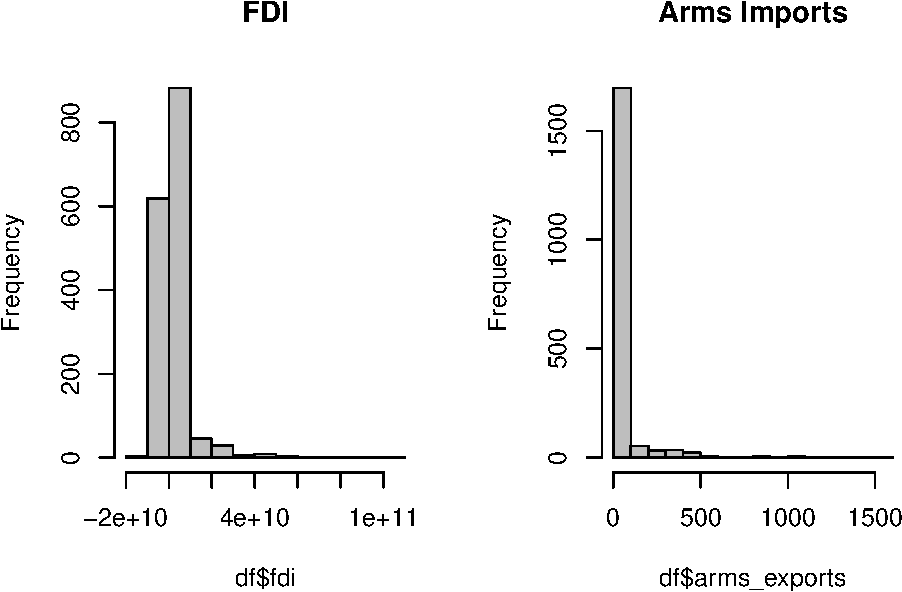
\includegraphics{proposal_files/figure-latex/unnamed-chunk-13-1.pdf}

It might make sense for modeling purposes to take the logs of these
variables, or at least of FDI---though some values are negative:

\begin{Shaded}
\begin{Highlighting}[]
\KeywordTok{par}\NormalTok{(}\DataTypeTok{mfrow=}\KeywordTok{c}\NormalTok{(}\DecValTok{1}\NormalTok{,}\DecValTok{2}\NormalTok{))}
\KeywordTok{hist}\NormalTok{(}\KeywordTok{log}\NormalTok{(df}\OperatorTok{$}\NormalTok{fdi), }\DataTypeTok{main=}\StringTok{'FDI Logged'}\NormalTok{, }\DataTypeTok{col=}\StringTok{'gray'}\NormalTok{)}
\end{Highlighting}
\end{Shaded}

\begin{verbatim}
## Warning in log(df$fdi): NaNs produced
\end{verbatim}

\begin{Shaded}
\begin{Highlighting}[]
\KeywordTok{hist}\NormalTok{(}\KeywordTok{log}\NormalTok{(df}\OperatorTok{$}\NormalTok{arms_exports), }\DataTypeTok{main=}\StringTok{'Arms Imports Logged'}\NormalTok{, }\DataTypeTok{col=}\StringTok{'gray'}\NormalTok{)}
\end{Highlighting}
\end{Shaded}

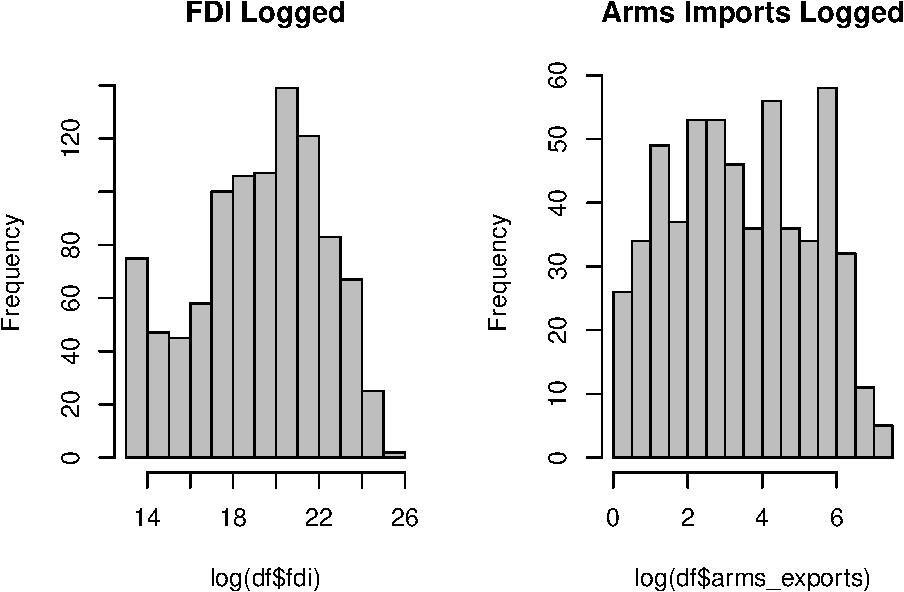
\includegraphics{proposal_files/figure-latex/unnamed-chunk-14-1.pdf}

The tremendous skew in FDI is obvious by comparing the mean and the
median, almost 2 billion and 10 million, respectively. Standard
deviation is also very high, almost 700 million.

\begin{Shaded}
\begin{Highlighting}[]
\KeywordTok{describe}\NormalTok{(df}\OperatorTok{$}\NormalTok{fdi)}
\end{Highlighting}
\end{Shaded}

\begin{verbatim}
## df$fdi 
##          n    missing   distinct       Info       Mean        Gmd 
##       1596        268        711      0.994  1.887e+09  3.764e+09 
##        .05        .10        .25        .50        .75        .90 
## -2.030e+08 -3.700e+07  0.000e+00  1.000e+07  6.820e+08  4.116e+09 
##        .95 
##  1.236e+10 
## 
## lowest : -19284000000 -15041000000  -9708000000  -8797000000  -8545000000
## highest:  50184000000  50230000000  51588000000  75007000000 109097000000
\end{verbatim}

It occurrs to me it might make sense to standardize FDI by dividing it
by a country's population or GDP---something to experiment with.

Just for fun, let's look at the top 10 recipients of FDI from the U.S.
(in millions of USD):

\begin{Shaded}
\begin{Highlighting}[]
\CommentTok{# df %>% group_by(country) %>%}
\CommentTok{#     summarize(fdi = sum(fdi)) %>%}
\CommentTok{#     mutate(fdi = fdi / 1000000) %>%}
\CommentTok{#     arrange(desc(fdi)) %>% }
\CommentTok{#     select(country, fdi) %>% }
\CommentTok{#     top_n(10) %>%}
\CommentTok{#     kable}
\end{Highlighting}
\end{Shaded}

Most are highly developed nations with large GDPs, half of them in
Europe.

Arms exports also has a much larger mean than median, the latter at 0,
i.e., over half of these year-country units received no arms from the
United States.

\begin{Shaded}
\begin{Highlighting}[]
\KeywordTok{describe}\NormalTok{(df}\OperatorTok{$}\NormalTok{arms_exports)}
\end{Highlighting}
\end{Shaded}

\begin{verbatim}
## df$arms_exports 
##        n  missing distinct     Info     Mean      Gmd      .05      .10 
##     1864        0      190    0.662    37.18    67.87      0.0      0.0 
##      .25      .50      .75      .90      .95 
##      0.0      0.0      4.0     87.7    272.0 
## 
## lowest :    0    1    2    3    4, highest: 1027 1110 1114 1389 1526
\end{verbatim}

The top 10 recipients of U.S. arms over this time period:

\begin{Shaded}
\begin{Highlighting}[]
\CommentTok{# df %>% group_by(country) %>%}
\CommentTok{#     summarize(arms_exports = sum(arms_exports )) %>%}
\CommentTok{#     arrange(desc(arms_exports )) %>% }
\CommentTok{#     select(country,arms_exports ) %>% }
\CommentTok{#     top_n(10) %>%}
\CommentTok{#     kable}
\end{Highlighting}
\end{Shaded}

This all looks correct. Israel is the largest recipient, and Egypt
receives tons of aid under the Camp David Treaty that President Carter
negotiated.

We can also examine some of the relationships between other independent
variables and FDI:

\begin{Shaded}
\begin{Highlighting}[]
\KeywordTok{ggplot}\NormalTok{(}\DataTypeTok{data=}\KeywordTok{na.omit}\NormalTok{(df), }\KeywordTok{aes}\NormalTok{(}\DataTypeTok{x=}\KeywordTok{as.factor}\NormalTok{(polity2), }\DataTypeTok{y=}\NormalTok{fdi}\OperatorTok{/}\DecValTok{1000000}\NormalTok{)) }\OperatorTok{+}
\StringTok{    }\KeywordTok{geom_bar}\NormalTok{(}\DataTypeTok{stat=}\StringTok{'identity'}\NormalTok{) }\OperatorTok{+}
\StringTok{    }\KeywordTok{ggtitle}\NormalTok{(}\StringTok{'FDI by Regime Type'}\NormalTok{)}
\end{Highlighting}
\end{Shaded}

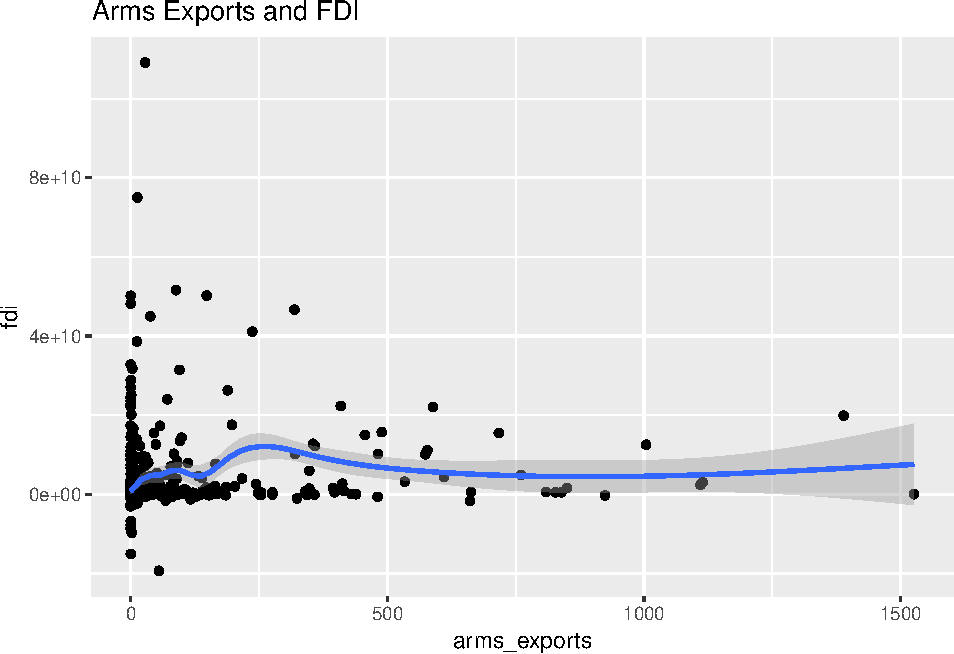
\includegraphics{proposal_files/figure-latex/unnamed-chunk-19-1.pdf}

The above makes it clear that most FDI goes to democratic countries
(Polity2 score of 8-10).

The same graph with arms exports suggests more variability, including a
more substantial portion to completely autocratic countries (-10).

\begin{Shaded}
\begin{Highlighting}[]
\KeywordTok{ggplot}\NormalTok{(}\KeywordTok{na.omit}\NormalTok{(df), }\KeywordTok{aes}\NormalTok{(}\DataTypeTok{x=}\KeywordTok{as.factor}\NormalTok{(polity2), }\DataTypeTok{y=}\NormalTok{arms_exports)) }\OperatorTok{+}\StringTok{ }
\StringTok{    }\KeywordTok{geom_bar}\NormalTok{(}\DataTypeTok{stat=}\StringTok{'identity'}\NormalTok{) }\OperatorTok{+}
\StringTok{    }\KeywordTok{ggtitle}\NormalTok{(}\StringTok{'Arms Exports by Regime Type'}\NormalTok{)}
\end{Highlighting}
\end{Shaded}

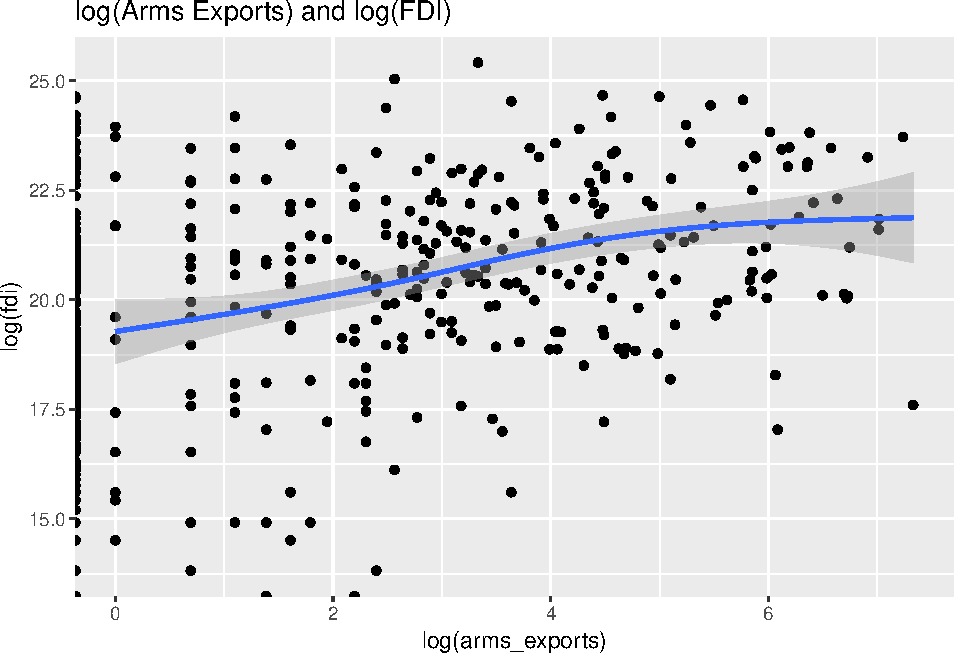
\includegraphics{proposal_files/figure-latex/unnamed-chunk-20-1.pdf}

Again, these may benefit by standardizing by population or GDP, or by
taking the log.

Finally, let's look at a scatterplot to view the direct relationship
between FDI and arms exports:

\begin{Shaded}
\begin{Highlighting}[]
\KeywordTok{ggplot}\NormalTok{(}\KeywordTok{na.omit}\NormalTok{(df), }\KeywordTok{aes}\NormalTok{(}\DataTypeTok{x=}\NormalTok{arms_exports, }\DataTypeTok{y=}\NormalTok{fdi)) }\OperatorTok{+}\StringTok{ }
\StringTok{    }\KeywordTok{geom_point}\NormalTok{() }\OperatorTok{+}
\StringTok{    }\KeywordTok{geom_smooth}\NormalTok{() }\OperatorTok{+}
\StringTok{    }\KeywordTok{ggtitle}\NormalTok{(}\StringTok{'Arms Exports and FDI'}\NormalTok{)}
\end{Highlighting}
\end{Shaded}

\begin{verbatim}
## `geom_smooth()` using method = 'gam' and formula 'y ~ s(x, bs = "cs")'
\end{verbatim}

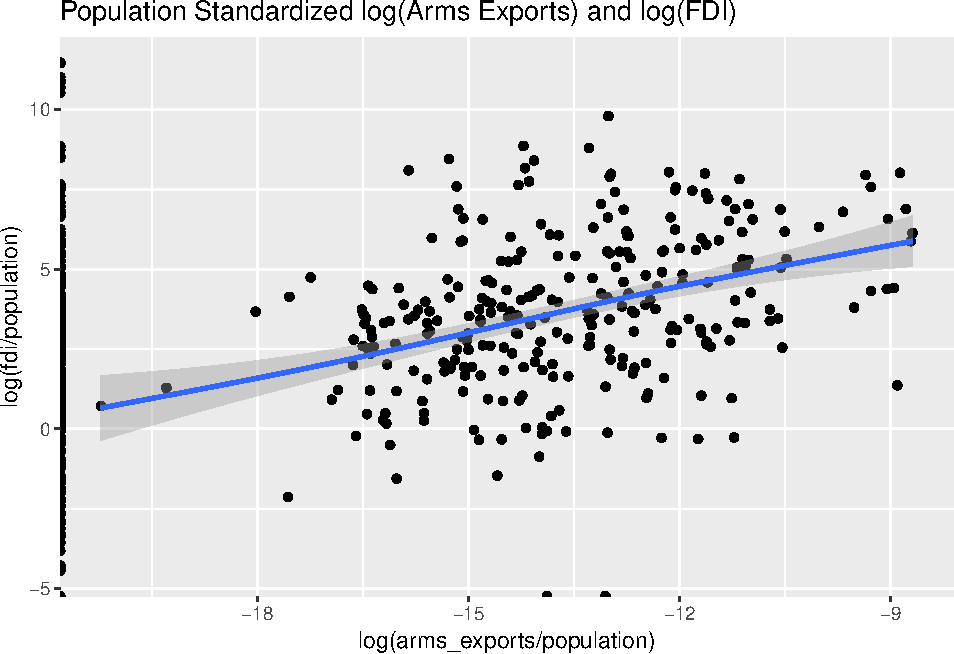
\includegraphics{proposal_files/figure-latex/unnamed-chunk-21-1.pdf}

Let's try taking the log of both variables:

\begin{Shaded}
\begin{Highlighting}[]
\KeywordTok{ggplot}\NormalTok{(}\KeywordTok{na.omit}\NormalTok{(df), }\KeywordTok{aes}\NormalTok{(}\DataTypeTok{x=}\KeywordTok{log}\NormalTok{(arms_exports), }\DataTypeTok{y=}\KeywordTok{log}\NormalTok{(fdi))) }\OperatorTok{+}\StringTok{ }
\StringTok{    }\KeywordTok{geom_point}\NormalTok{() }\OperatorTok{+}
\StringTok{    }\KeywordTok{geom_smooth}\NormalTok{() }\OperatorTok{+}
\StringTok{    }\KeywordTok{ggtitle}\NormalTok{(}\StringTok{'log(Arms Exports) and log(FDI)'}\NormalTok{)}
\end{Highlighting}
\end{Shaded}

\begin{verbatim}
## Warning in log(fdi): NaNs produced

## Warning in log(fdi): NaNs produced

## Warning in log(fdi): NaNs produced
\end{verbatim}

\begin{verbatim}
## `geom_smooth()` using method = 'gam' and formula 'y ~ s(x, bs = "cs")'
\end{verbatim}

\begin{verbatim}
## Warning: Removed 748 rows containing non-finite values (stat_smooth).
\end{verbatim}

\begin{verbatim}
## Warning: Removed 244 rows containing missing values (geom_point).
\end{verbatim}

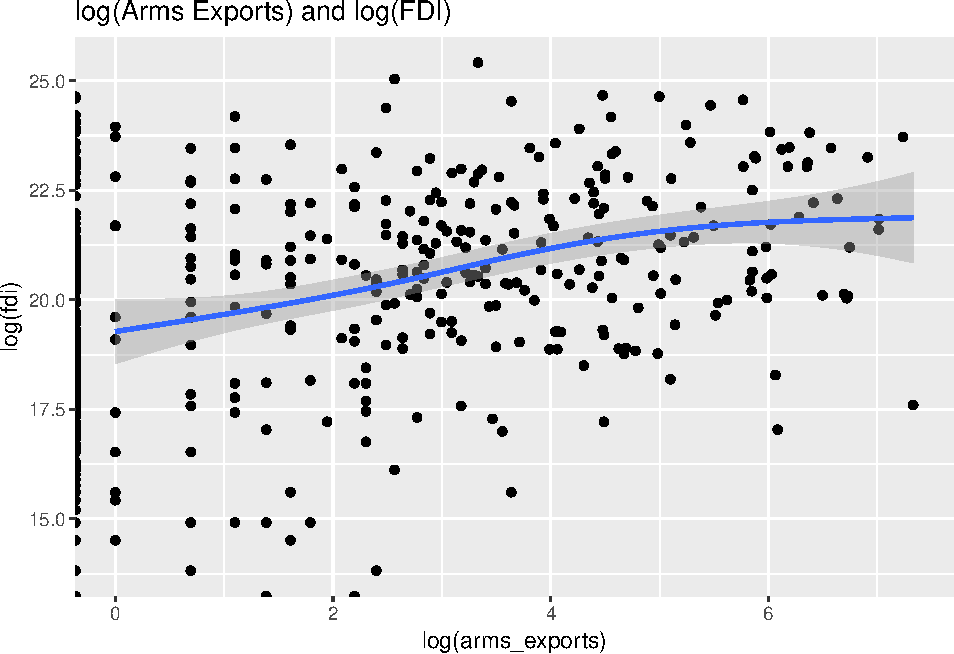
\includegraphics{proposal_files/figure-latex/unnamed-chunk-22-1.pdf}

This looks much better! Let's just try one more, dividing both values by
population and then taking the log:

\begin{Shaded}
\begin{Highlighting}[]
\KeywordTok{ggplot}\NormalTok{(}\KeywordTok{na.omit}\NormalTok{(df), }\KeywordTok{aes}\NormalTok{(}\DataTypeTok{x=}\KeywordTok{log}\NormalTok{(arms_exports}\OperatorTok{/}\NormalTok{population), }\DataTypeTok{y=}\KeywordTok{log}\NormalTok{(fdi}\OperatorTok{/}\NormalTok{population))) }\OperatorTok{+}\StringTok{ }
\StringTok{    }\KeywordTok{geom_point}\NormalTok{() }\OperatorTok{+}
\StringTok{    }\KeywordTok{geom_smooth}\NormalTok{() }\OperatorTok{+}
\StringTok{    }\KeywordTok{ggtitle}\NormalTok{(}\StringTok{'Population Standardized log(Arms Exports) and log(FDI)'}\NormalTok{)}
\end{Highlighting}
\end{Shaded}

\begin{verbatim}
## Warning in log(fdi/population): NaNs produced

## Warning in log(fdi/population): NaNs produced

## Warning in log(fdi/population): NaNs produced
\end{verbatim}

\begin{verbatim}
## `geom_smooth()` using method = 'gam' and formula 'y ~ s(x, bs = "cs")'
\end{verbatim}

\begin{verbatim}
## Warning: Removed 748 rows containing non-finite values (stat_smooth).
\end{verbatim}

\begin{verbatim}
## Warning: Removed 244 rows containing missing values (geom_point).
\end{verbatim}

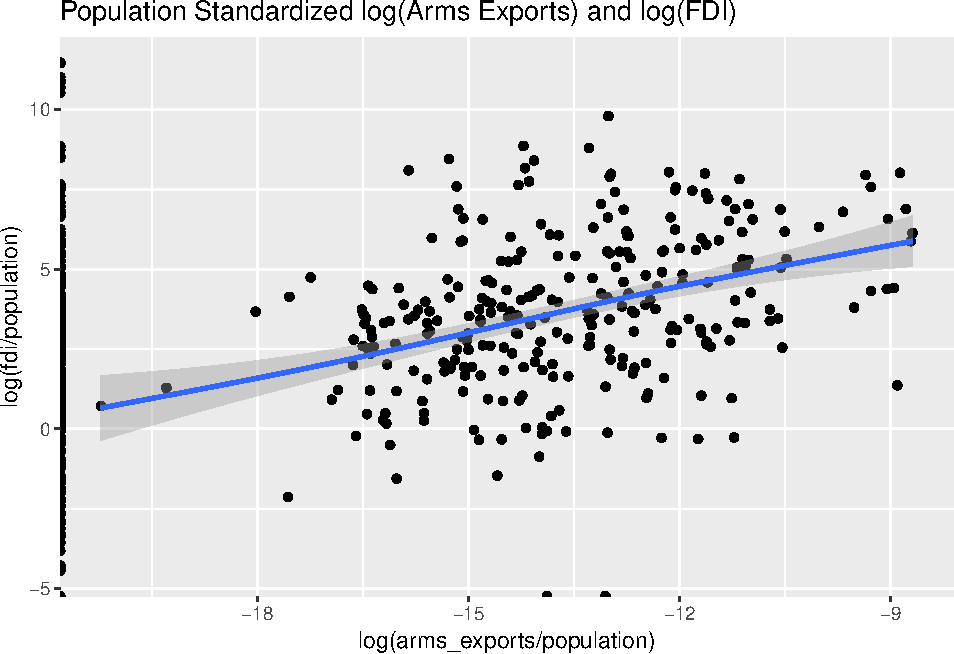
\includegraphics{proposal_files/figure-latex/unnamed-chunk-23-1.pdf}

BEAUTIFUL. This graph actually looks so good I feel like I've cheated
somewhere?! But I'll have to drop population as an explantory variable,
though.

\hypertarget{misc.-notes}{%
\section{Misc. Notes}\label{misc.-notes}}

\hypertarget{todo}{%
\subsection{TODO}\label{todo}}

\begin{enumerate}
\def\labelenumi{\arabic{enumi}.}
\item
  Create some kind of mapping of countries so that more of them get
  passed all the joins.
\item
  Consider some strategies to fill in missing values. E.g., Polity does
  not assign a regime for Afghanistan for several years because of the
  conflict there---what makes sense as a way to handle this reasonably
  without just dropping the rows?
\item
  Fill NAs with zeros where necessary.
\item
  Attempt three models: regular \texttt{lm}, \texttt{plm} for panel
  data, and the original two-step least squares, paying particular
  attention to showing the violation of \texttt{lm} assumptions and how
  the latter two correct this.
\end{enumerate}

\hypertarget{modeling}{%
\subsection{Modeling}\label{modeling}}

Note on two-stage least squares regression:

\begin{enumerate}
\def\labelenumi{\arabic{enumi}.}
\tightlist
\item
  Authors first developed a \emph{troop} model:
\end{enumerate}

\[troops \sim conflict_{-1} + alliance_{-1} + polity_{-1} + warsaw\_pact_{-1} + cold\_war_{-1} + log(pop_{-1}) + reagan_{-1} + south_korea + vietnam + philippines\]

\begin{enumerate}
\def\labelenumi{\arabic{enumi}.}
\setcounter{enumi}{1}
\tightlist
\item
  Then plugged the results of that model into a \emph{trade} model with
  some other variables:
\end{enumerate}

\[trade \sim troops + growth_{-1} + gdp_{-1} + distance + alliance_{-1}\]

\begin{itemize}
\tightlist
\item
  both models including intercepts
\end{itemize}


\end{document}
